\documentclass[10pt]{article}

\usepackage{geometry}
\geometry{margin=3em,top=6em, left=2.5cm, headheight=\paperheight}
\usepackage[export]{adjustbox}
\usepackage{array}
\usepackage{amsmath}
\usepackage{amsfonts}
\usepackage{fancyhdr}
\pagestyle{fancy}
\fancyhf{}
\lhead{Algebra II}
\chead{Increasing/Decreasing}
\rhead{Practice, Page \thepage}
\usepackage{lastpage}
\usepackage{xcolor}
\usepackage{enumitem}
\usepackage{pifont}
\usepackage{graphicx}
\graphicspath{{../img}}
\usepackage{pgfplots}
\pgfplotsset{compat=1.18}
\usepackage{tabularx}

\newcommand{\R}{\mathbb R}
\newcommand{\e}{{\rm e}}
\newcommand{\pobr}[1]{\left\langle#1\right\rangle}
\newcommand{\norm}[1]{\lVert #1 \rVert}
\newcommand{\abs}[1]{\lvert #1 \rvert}

\DeclareMathOperator{\xd}{d\!}
\DeclareMathOperator{\proj}{proj}

\title{}
\date{}

\begin{document}
\noindent
{
Name \rule{16em}{.5pt}\hspace{\stretch{1}} Date \rule{8em}{.5pt}\hspace{\stretch{1}} Period \rule{4em}{.5pt}
}
\vspace{1em}

{\noindent\bf Targets.}
\begin{itemize}
    \item to convert between inequalities and intervals.
    \item to determine the increasing/decreasing intervals of a graph.
\end{itemize}
{\noindent\bf Do Now.}
\begin{enumerate}
    \item How do you use the word {\it increasing/decreasing} in everyday life?
    \vspace{\stretch{1}}
    
    \item How would you draw a graph that is {\it increasing} according to your common sense?
\begin{center}
    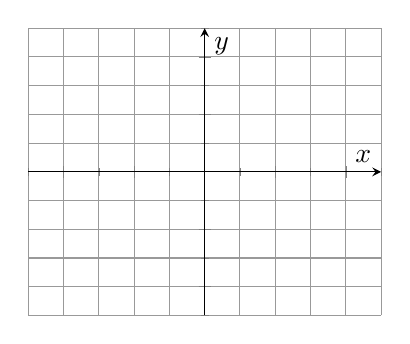
\begin{tikzpicture}
\begin{axis}[
    xlabel={$x$},
    ylabel={$y$},
    grid=both,
    minor tick num=1,
    axis lines=middle,
    xmin=-5,xmax=5,
    ymin=-5,ymax=5,
    domain=-5:5,
    samples=100,
    width=0.5\textwidth,
    grid style={draw=gray!80},
    xticklabels=\empty,
    yticklabels=\empty
]
\end{axis}
\end{tikzpicture}
\end{center}    

\end{enumerate}

{\noindent\bf Take note.}\\[1em]

\noindent
\rule{\textwidth}{.1pt}\\[1.5em]
\rule{\textwidth}{.1pt}\\[1.5em]
\rule{\textwidth}{.1pt}\\[1.5em]
\rule{\textwidth}{.1pt}\\[1.5em]
\rule{\textwidth}{.1pt}\\[1.5em]
\rule{\textwidth}{.1pt}\\[1.5em]
\rule{\textwidth}{.1pt}\\[1.5em]
\rule{\textwidth}{.1pt}\\[1.5em]
\rule{\textwidth}{.1pt}\\[1.5em]
\rule{\textwidth}{.1pt}\\[1.5em]

\clearpage

{\noindent\bf Practice.}
\begin{enumerate}
    \item Convert the inequality to an interval: \(-5<x\leq4\). \rule{8em}{0.5pt}
    \vspace{\stretch{1}}


    \item Convert the interval to an inequality: \([8, \infty)\). \rule{8em}{0.5pt}
    \vspace{\stretch{1}}

\end{enumerate}

{\noindent\bf Discussion.}
Does a constantly increasing function necessarily approach positive infinity eventually? Draw one and show your neighbors.
\begin{center}
    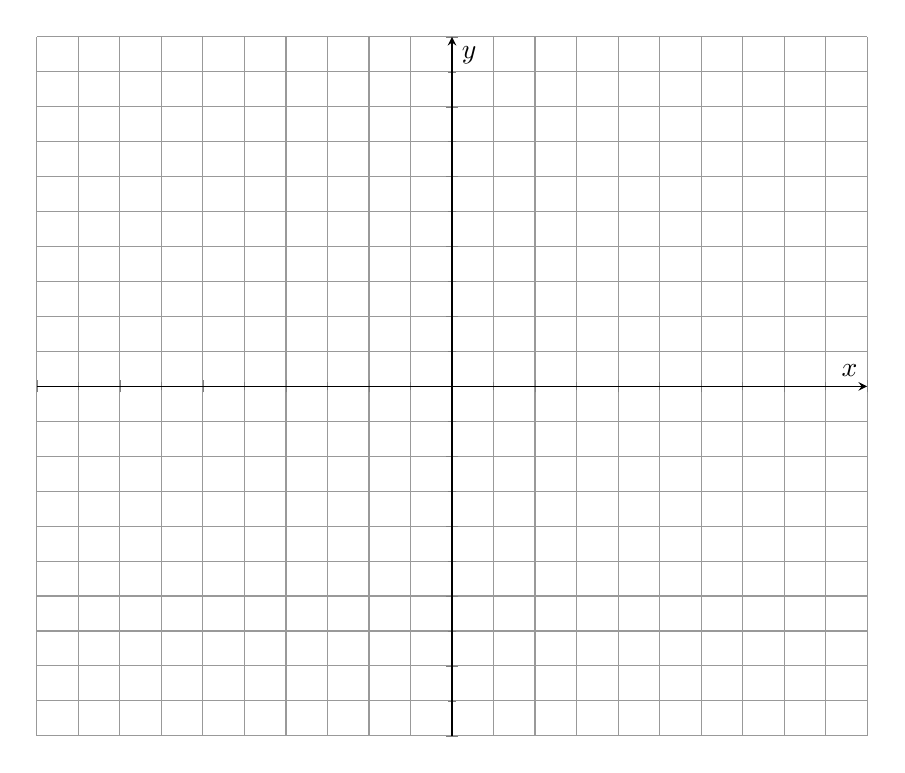
\begin{tikzpicture}
\begin{axis}[
    xlabel={$x$},
    ylabel={$y$},
    grid=both,
    minor tick num=1,
    axis lines=middle,
    xmin=-5,xmax=5,
    ymin=-5,ymax=5,
    domain=-5:5,
    samples=100,
    width=\textwidth,
    grid style={draw=gray!80},
    xticklabels=\empty,
    yticklabels=\empty
]
\end{axis}
\end{tikzpicture}
\end{center}
\vspace{\stretch{1}}


\end{document}